../cictikz/src/cictikz/data/tex/cictikz_preamble.tex

% De Morgan: the two truth tables prove the identities, and the two
% cautions on the right are the mistakes everyone makes once.

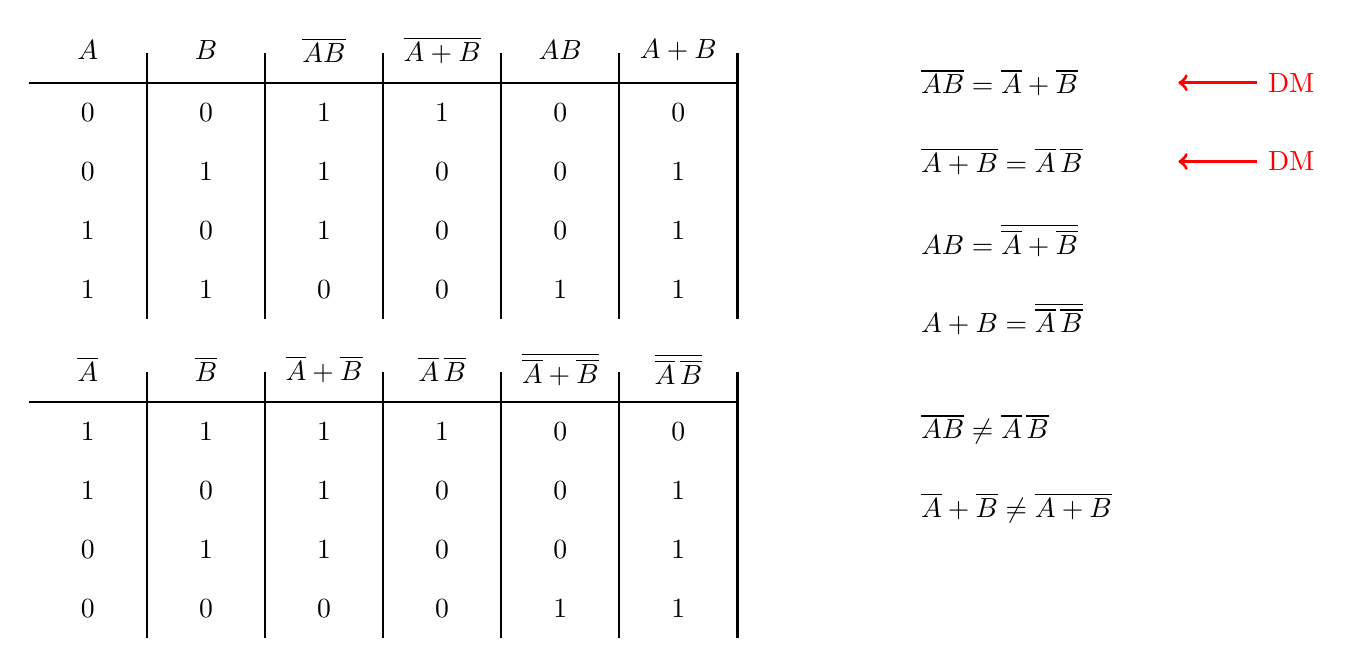
\begin{tikzpicture}[thick]

  \def\cw{1.5}   % column width
  \def\rh{0.75}  % row height

  % ----------------------------------------------------------------
  % Table 1: A, B, /(AB), /(A+B), AB, A+B
  % ----------------------------------------------------------------
  \begin{scope}[shift={(0,0)}]
    % vertical lines (between columns, and after the last)
    \foreach \i in {1,...,6} {
      \draw ({\i*\cw},{0.5*\rh}) -- ({\i*\cw},{-4*\rh});
    }
    % horizontal line under the header
    \draw (0,0) -- ({6*\cw},0);

    % header
    \node at ({0.5*\cw},{0.55*\rh}) {$A$};
    \node at ({1.5*\cw},{0.55*\rh}) {$B$};
    \node at ({2.5*\cw},{0.55*\rh}) {$\overline{AB}$};
    \node at ({3.5*\cw},{0.55*\rh}) {$\overline{A+B}$};
    \node at ({4.5*\cw},{0.55*\rh}) {$AB$};
    \node at ({5.5*\cw},{0.55*\rh}) {$A+B$};

    % rows
    \foreach \r/\va/\vb/\vc/\vd/\ve/\vf in {%
      1/0/0/1/1/0/0,
      2/0/1/1/0/0/1,
      3/1/0/1/0/0/1,
      4/1/1/0/0/1/1}{
      \node at ({0.5*\cw},{-(\r-0.5)*\rh}) {\va};
      \node at ({1.5*\cw},{-(\r-0.5)*\rh}) {\vb};
      \node at ({2.5*\cw},{-(\r-0.5)*\rh}) {\vc};
      \node at ({3.5*\cw},{-(\r-0.5)*\rh}) {\vd};
      \node at ({4.5*\cw},{-(\r-0.5)*\rh}) {\ve};
      \node at ({5.5*\cw},{-(\r-0.5)*\rh}) {\vf};
    }
  \end{scope}

  % ----------------------------------------------------------------
  % Table 2: /A, /B, /A+/B, /A/B, /(/A+/B), /(/A/B)
  % ----------------------------------------------------------------
  \begin{scope}[shift={(0,{-5.4*\rh})}]
    \foreach \i in {1,...,6} {
      \draw ({\i*\cw},{0.5*\rh}) -- ({\i*\cw},{-4*\rh});
    }
    \draw (0,0) -- ({6*\cw},0);

    \node at ({0.5*\cw},{0.55*\rh}) {$\overline{A}$};
    \node at ({1.5*\cw},{0.55*\rh}) {$\overline{B}$};
    \node at ({2.5*\cw},{0.55*\rh}) {$\overline{A}+\overline{B}$};
    \node at ({3.5*\cw},{0.55*\rh}) {$\overline{A}\,\overline{B}$};
    \node at ({4.5*\cw},{0.55*\rh}) {$\overline{\overline{A}+\overline{B}}$};
    \node at ({5.5*\cw},{0.55*\rh}) {$\overline{\overline{A}\,\overline{B}}$};

    \foreach \r/\va/\vb/\vc/\vd/\ve/\vf in {%
      1/1/1/1/1/0/0,
      2/1/0/1/0/0/1,
      3/0/1/1/0/0/1,
      4/0/0/0/0/1/1}{
      \node at ({0.5*\cw},{-(\r-0.5)*\rh}) {\va};
      \node at ({1.5*\cw},{-(\r-0.5)*\rh}) {\vb};
      \node at ({2.5*\cw},{-(\r-0.5)*\rh}) {\vc};
      \node at ({3.5*\cw},{-(\r-0.5)*\rh}) {\vd};
      \node at ({4.5*\cw},{-(\r-0.5)*\rh}) {\ve};
      \node at ({5.5*\cw},{-(\r-0.5)*\rh}) {\vf};
    }
  \end{scope}

  % ----------------------------------------------------------------
  % Identities on the right
  % ----------------------------------------------------------------
  \begin{scope}[shift={(11.2,0)}]
    \node[anchor=west] (e1) at (0,0)     {$\overline{AB} = \overline{A}+\overline{B}$};
    \node[anchor=west] (e2) at (0,-1.0)  {$\overline{A+B} = \overline{A}\,\overline{B}$};
    \node[anchor=west] (e3) at (0,-2.0)  {$AB = \overline{\overline{A}+\overline{B}}$};
    \node[anchor=west] (e4) at (0,-3.0)  {$A+B = \overline{\overline{A}\,\overline{B}}$};

    \node[anchor=west] (e5) at (0,-4.4)  {$\overline{AB} \neq \overline{A}\,\overline{B}$};
    \node[anchor=west] (e6) at (0,-5.4)  {$\overline{A}+\overline{B} \neq \overline{A+B}$};

    % the two De Morgan identities, marked
    \draw[red, very thick, <-] (3.4,0)  -- (4.4,0)  node[anchor=west] {DM};
    \draw[red, very thick, <-] (3.4,-1.0) -- (4.4,-1.0) node[anchor=west] {DM};
  \end{scope}

\end{tikzpicture}
\end{document}
